\chapter{The Video Face Clustering Method}
\label{chap:video_face_clustering}

The core of this dissertation is a method that called \emph{Video Face Clustering}.
%%
It consists in detecting and grouping faces from different video frames~(ideally from the same actors) extracted from a video file.
%%
Figure \ref{fig:video_face_clustering} depicts this process, and each of its steps are described in the next paragraphs.

\begin{figure*}[!ht]
    \centering
    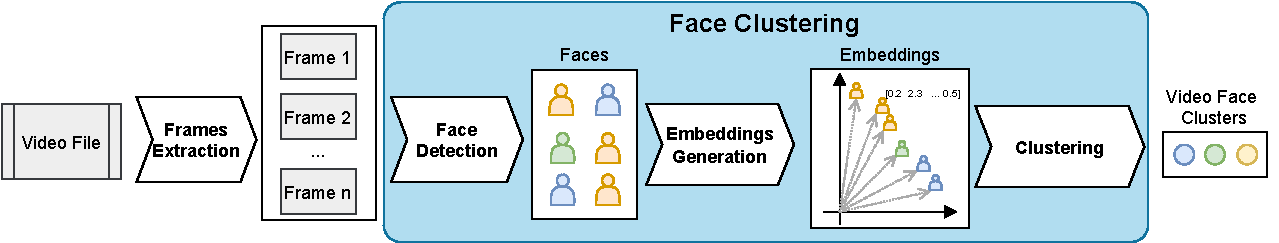
\includegraphics[width=\textwidth]{img/face_clustering/video_face_clustering.pdf}
    \caption{Video face clustering process.}
    \label{fig:video_face_clustering}
\end{figure*}


First, we perform \textit{Frames Extraction} by receiving a video file as input and extracting its frames according to a given frame rate. 
%%
These frames are used as a set of images for the next step.

The \textit{Face Detection} step uses an object detection model for detecting faces in each of its images.
%%
In general, any object detection model can identify which, among a known set of objects, are present in the image, and provides information about their positions.
%%
In our case, objects are faces and, therefore, the face detection model is responsible for returning the bounding boxes of the faces present in the image, specified by the $x$ and $y$ axes coordinates of the upper-left corner and of the lower-right corner of the rectangle that establishes the visual limits that encapsulate each face. 
%%
With these bounding boxes, we can isolate and extract the bounded images, obtaining a dataset composed of images of faces only.


The objective of the \textit{Embeddings Generation} step is to represent each face image as a vector space in $\mathbb{R}^{n}$.
%%
To achieve that, it processes each of the faces generated in the previous step through a CNN, generating embeddings. 
%%
An embedding is a representation of the input in a lower dimensional space.
%%
Ideally, an embedding captures some semantics of the input, e.g. by placing semantically similar inputs close together in the embedding space.
%
At the end of this step, we have all faces represented as embeddings.
%%

In the \textit{Clustering} step, we group embeddings and, consequently, faces that are close in the embedding space using a clustering algorithm. 
%
Clustering is the task of dividing a set of data points, embeddings in this case, into a number of groups~(clusters) such that data points in a given group are similar to other data points in the same group and dissimilar to the data points in other groups.
%%
The clustering process should produce a partition of the dataset, i.e., each generated cluster represents a specific person, and the union of all clusters covers the whole dataset.

By the end of this process, we expect to have the spatiotemporal localization of the actors present in a video file.
%%
Figure \ref{fig:timeline} shows an example of the results achieved by this method. It contains a timeline of a video with lines coloring the segments that each actor appears.

\begin{figure}[!ht]
    \centering
    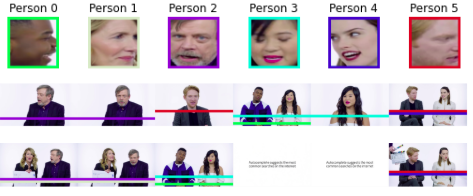
\includegraphics[width=0.6\linewidth]{img/face_clustering/timeline2.png}
    \caption{Timeline with tagged frames by their clusters}
    \label{fig:timeline}
\end{figure}

